%
% l1konvergenz.tex
%
% (c) 2023 Prof Dr Andreas Müller
%
\begin{figure}
\centering
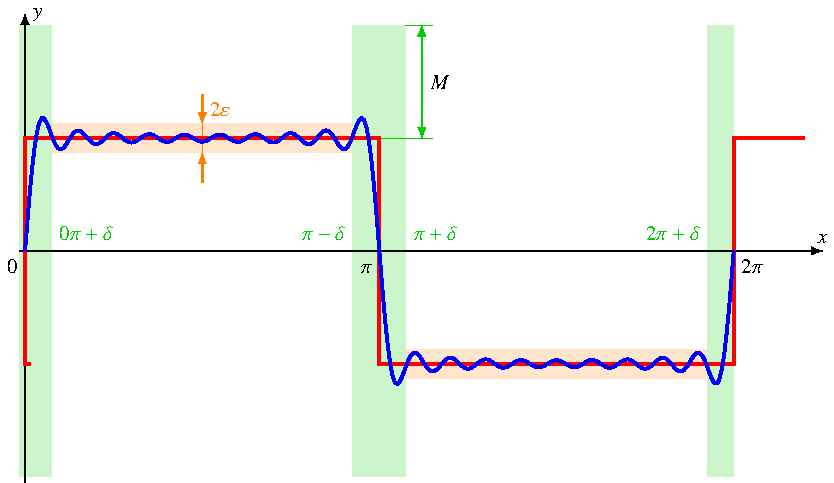
\includegraphics{chapters/010-skalarprodukt/images/l1konvergenz.pdf}
\caption{Konvergenz der Folge $f_n$ von
\eqref{buch:skalarprodukt:eqn:rechteckreihe} in der $L^1$-Norm.
Die $L^1$-Norm von $f_n-f$ ist beschränkt durch die farbige Fläche,
sie kann beliebig klein gemacht werden, indem $\varepsilon$ und
$\delta$ klein gewählt werden.
\label{buch:skalarprodukt:funktionenraeume:fig:l1konvergenz}}
\end{figure}
